\section{Background}

In this section we present background information about the NVMe interface and
the SPDK framework. We also present testFS, a user space file system that our
file system is based on.

\subsection{NVMe and I/O Queues}

NVMe~\cite{nvme} is an open interface specification designed to allow host
software to communicate with a non-volatile memory subsystem (NVM) via a
peripheral component interconnect express (PCIe) bus. Previous standards such
as serial-attached SCSI and serial advanced technology attachment (SATA) can
handle queue depths of 254 and 32 respectively. NVMe is able to handle queue
depths of up to 65535 I/O queues with up to 64 Ki outstanding commands per I/O
queue~\cite{nvme}, which allows an NVMe device to support parallel operations.
An I/O queue is composed of a submission queue and a completion queue. Host
software issues I/O commands to a submission queue and completions are placed
into the associated completion queue by the controller. Note that the order of
completions is not determined by the submission order of the commands.

\subsection{SPDK and Block Devices}

SPDK~\cite{spdk} is an open source library that allows developers to implement
high performance, scalable, user-mode storage applications. A block device in
SPDK is an abstraction over all block devices. I/O commands are processed and
issued to corresponding physical block devices such as NVMe devices and memory
allocated devices. SPDK provides a event framework, where different threads
can exchange data by sending messages to each other. SPDK enables developers to
build asynchronous, lockless, and high performance applications.

\begin{figure}
  \centering
  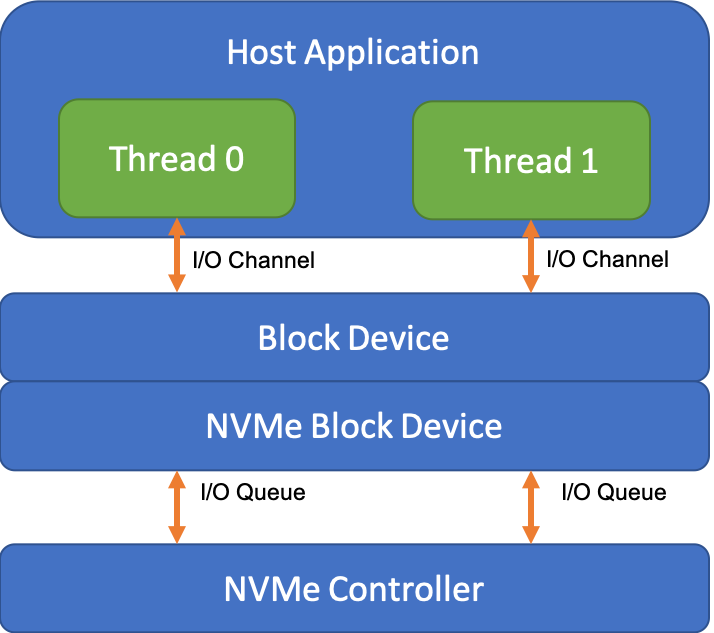
\includegraphics[height=6cm]{spdk_arch}
  \caption{Example of an SPDK application.}
  \label{fig:spdk_arch}
\end{figure}

SPDK uses an I/O channel to represent the channel for accessing an I/O device.
I/O channels are tied to a specific thread, so a distinct I/O channel is
created per thread. I/O requests issued to the block device are forwarded to
the underlying physical device. In our implementation, an I/O channel
corresponds to an I/O queue of the underlying NVMe device. The framework builds
I/O commands based on I/O requests and submits them to the device's submission
queue. It then polls for I/O completions on each queue pair with outstanding
I/O to receive completion callbacks. Figure~\ref{fig:spdk_arch} provides a
graphical representation of a host application using SPDK block devices to
interact with an NVMe device. In the host application, each thread submits I/O
requests to its corresponding I/O channel. The I/O channel forwards the I/O
requests to the actual physical device based on the implementation of the
physical block device. The framework invokes a callback function when the I/O
request completes.

\subsection{TestFS}

TestFS\cite{testfs} is a user space file system which is similar to {\tt
  ext3}~\cite{ext3}, a journaled file system that is commonly used by the Linux
kernel. TestFS has three levels of indirection, which are illustrated in
Figure~\ref{fig:testfs}. A super block points to metadata and an inode block of
the root directory. The metadata stores the block freemap as well as the
checksum of the data blocks. Inode blocks point to data blocks where the actual
data is stored. In testFS, both directory data and indirect inode data are
stored in data blocks. The space assigned to inode blocks and data blocks is
pre-allocated and fixed during the life cycle of testFS.

Note that our file system is based on testFS because testFS is well-maintained,
user level, and well-documented. Extending testFS allows us to build a proof of
concept of our design quickly. We believe our modifications to testFS can be
applied to most other file systems as well.

\begin{figure}[h!]
  \centering
  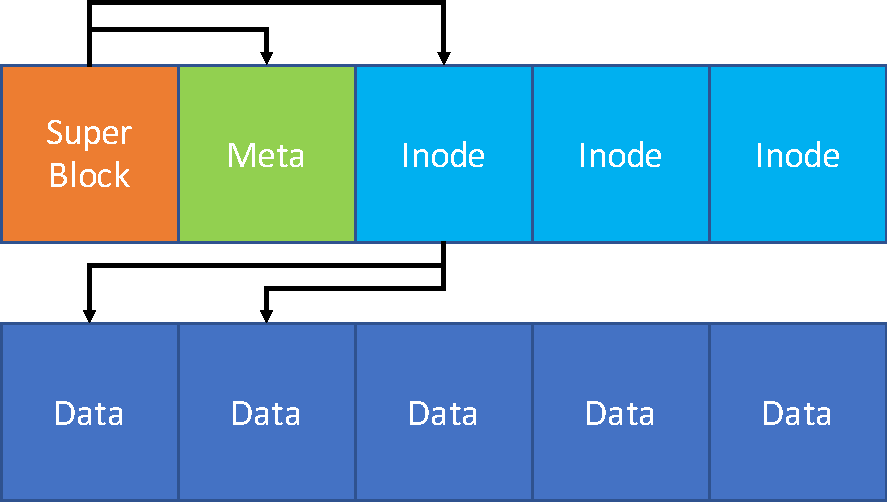
\includegraphics[height=4cm]{testfs}
  \caption{The layout of blocks with different types in testFS.}
  \label{fig:testfs}
\end{figure}
